\documentclass[]{article}
\usepackage[T1]{fontenc}
\usepackage{lmodern}
\usepackage{amssymb,amsmath}
\usepackage{ifxetex,ifluatex}
\usepackage{fixltx2e} % provides \textsubscript
% use upquote if available, for straight quotes in verbatim environments
\IfFileExists{upquote.sty}{\usepackage{upquote}}{}
\ifnum 0\ifxetex 1\fi\ifluatex 1\fi=0 % if pdftex
  \usepackage[utf8]{inputenc}
\else % if luatex or xelatex
  \ifxetex
    \usepackage{mathspec}
    \usepackage{xltxtra,xunicode}
  \else
    \usepackage{fontspec}
  \fi
  \defaultfontfeatures{Mapping=tex-text,Scale=MatchLowercase}
  \newcommand{\euro}{€}
\fi
% use microtype if available
\IfFileExists{microtype.sty}{\usepackage{microtype}}{}
\usepackage{graphicx}
% Redefine \includegraphics so that, unless explicit options are
% given, the image width will not exceed the width of the page.
% Images get their normal width if they fit onto the page, but
% are scaled down if they would overflow the margins.
\makeatletter
\def\ScaleIfNeeded{%
  \ifdim\Gin@nat@width>\linewidth
    \linewidth
  \else
    \Gin@nat@width
  \fi
}
\makeatother
\let\Oldincludegraphics\includegraphics
{%
 \catcode`\@=11\relax%
 \gdef\includegraphics{\@ifnextchar[{\Oldincludegraphics}{\Oldincludegraphics[width=\ScaleIfNeeded]}}%
}%
\ifxetex
  \usepackage[setpagesize=false, % page size defined by xetex
              unicode=false, % unicode breaks when used with xetex
              xetex]{hyperref}
\else
  \usepackage[unicode=true]{hyperref}
\fi
\hypersetup{breaklinks=true,
            bookmarks=true,
            pdfauthor={Rob Murrer},
            pdftitle={Enhanced 8-Puzzle Genetic Algorithm},
            colorlinks=true,
            citecolor=blue,
            urlcolor=blue,
            linkcolor=magenta,
            pdfborder={0 0 0}}
\urlstyle{same}  % don't use monospace font for urls
\setlength{\parindent}{0pt}
\setlength{\parskip}{6pt plus 2pt minus 1pt}
\setlength{\emergencystretch}{3em}  % prevent overfull lines
\setcounter{secnumdepth}{0}

\title{Enhanced 8-Puzzle Genetic Algorithm}
\author{Rob Murrer}
\date{March 11, 2014}

\begin{document}
\maketitle

\section{Introduction}\label{introduction}

This project is a continuation of a previous assignment. The original
Genetic Algorithm (GA) has been modified significantly. These changes
include the implementation of selection and crossover as well as a
logging function that allows graphs to be made of the run of the GA.
These graphs proved invaluable in understanding and tuning the Baseline
GA (BLGA).

\begin{figure}[htbp]
\centering
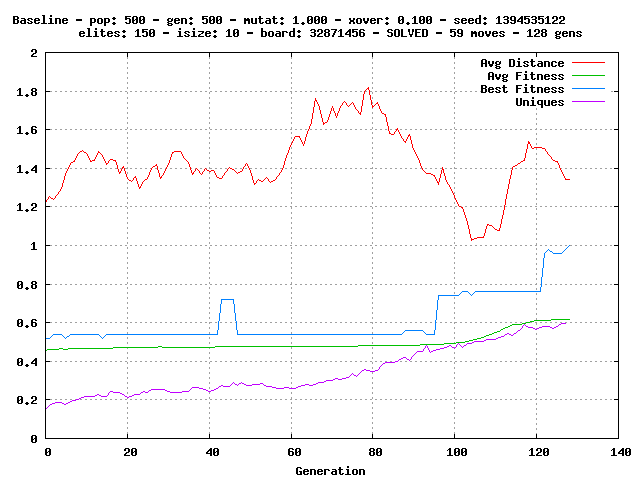
\includegraphics{img/intro-graph.png}
\caption{Example Graph of GA Run}
\end{figure}

A couple of population diversity measurements were created to analyze
the BLGA. These measurements were used to create an Enhanced GA (ENGA).
The ENGA uses the diversity measurement to influence the GA.

The comparison in performance by the BLGA and the ENGA was measured in
the number of generations needed to solve a puzzle and the size of the
solution. The ENGA performed better than the BLGA in solution size but
performed worse in the number of generations needed.

\section{Baseline Genetic Algorithm}\label{baseline-genetic-algorithm}

\subsection{Problem Representation}\label{problem-representation}

A solution to an 8 puzzle problem can be represented as a series of
changes in tile positions. A single state of the puzzle in this Genetic
Algorithm (GA) is represented by a single 32 bit integer. The encoding
of the state of the puzzle is a simple reading of the numbers in cells 1
to 9 and combining them into a single integer. For example the following
board is encoded as 321456078.

\begin{verbatim}
3 2 1
4 5 6
0 7 8
\end{verbatim}

A solution is an ordered list of these board positions. Internally it is
implemented as a doubly linked list and a hash table for fast lookup.

\subsection{Initialization of
Population}\label{initialization-of-population}

There is an initial growth to the population that is not considered part
of the GA. There is a constant value (30 in this case) that each
solution will mutate before the run starts. The solutions are grown from
the initial tile state.

\subsection{Selection Algorithm}\label{selection-algorithm}

The population is sorted according to fitness. The elite members are
then paired with the other members of the population.

\subsection{Crossover Algorithm}\label{crossover-algorithm}

A single point crossover method is used. The elite chromosome is
iterated from the current state to the first state. At each position a
search is done in the weaker chromosome for a matching position in the
elite. The elite chromosome will then be copied to the weaker at that
point. The left half of the new chromosome will be from the weaker and
the right half will be from the elite. All chromosomes have at least one
crossover point, the original board configuration.

\subsection{Mutation Algorithm}\label{mutation-algorithm}

There are 4 ways a chromosome can mutate. In each method steps are taken
to never create a cycle. Randomly one of the following are applied on
each mutation call:

\begin{enumerate}
\itemsep1pt\parskip0pt\parsep0pt
\item
  Grow one new move to increase fitness value
\item
  Grow one new move to a random non-cycling position
\item
  Modify current board state into random non-cycling position
\item
  If larger than 31 moves then truncate to a random length else nothing
\end{enumerate}

\subsection{Fitness Function}\label{fitness-function}

A Manhattan distance and the correctness of the top row and left columns
are used in the fitness function. The Manhattan distance is the sum of
the total distance horizontally and vertically to the tiles goal
state.\\The fitness value for a solution is calculated by this formula
applied to the current state of the solution:

\begin{verbatim}
Fitness = 1 - Manhattan*0.01 - TopLeft*0.2
\end{verbatim}

\subsection{Parameters of GA}\label{parameters-of-ga}

These parameters will solve most 8 puzzles in under 150 generations.

\begin{itemize}
\itemsep1pt\parskip0pt\parsep0pt
\item
  \texttt{population size}: 500
\item
  \texttt{number of generations}: 500
\item
  \texttt{mutation probability}: 1.0
\item
  \texttt{crossover probability}: 0.10
\item
  \texttt{random seed}: time(0)
\item
  \texttt{initial size of solution}: 30
\item
  \texttt{elites}: 150
\end{itemize}

\section{Enhanced Genetic Algorithm}\label{enhanced-genetic-algorithm}

To ensure a fair comparison between the ENGA and the BLGA, the
parameters of the GA remained the same. A method for measuring the
Manhattan distance between each individual in the population was created
and used for visualization. This method proved too computationally
expensive to leave in the final version of the project. Instead a
quicker method for determining diversity was developed.

\subsection{Diversity Measurement}\label{diversity-measurement}

Each individual in the population was analyzed and counted to determine
the number of unique solutions in the population. This is done with a
simple hash-table counting method. At the beginning of each generation
in the population this calculation is done.

\subsection{Controlling Diversity}\label{controlling-diversity}

There are two parameters use to control diversity in the run: maximum
number of duplicates and hyper-mutation. Before the mutation and
crossover operations are done on the population, the population's
solutions were enumerated and checked against the maximum number of
duplicates.

If a solution was present in the population more than the maximum
allowed, the solutions that were greater than the maximum were
hyper-mutated. This hyper-mutations simply called the mutation operator
on the solution N times. N being the parameter hyper-mutation.

\section{Experiments}\label{experiments}

A number of experiments were run for tuning the BLGA before the
comparison to the ENGA. These experiments were simply optimizing the
parameters for a balance of solution size and generations needed to
complete the run. When the optimizations were made the parameters were
locked between the BLGA and ENGA.

\subsection{Tuning the ENGA}\label{tuning-the-enga}

In order to compare the ENGA to the BLGA the same random seed was chosen
for both during tuning. The hyper-mutation parameter was modified in 25
percent increments and decrements until the value of 100 was found to be
outperforming the BLGA. The maximum number of duplicates allowed were
optimized in the same way. Maximum number of duplicates was determined
to be ten percent of population.

\subsection{Comparing BLGA to ENGA}\label{comparing-blga-to-enga}

Randomness plays an important role in the function of both GAs so the
random seed was seeded with \texttt{time(0)} to prevent an artificial
bias from being created. Both GAs were run with two different initial
board configurations ten different times. The number of generations
needed and the solution size were averaged over the run of the
experiment

\subsubsection{Sampling of Data}\label{sampling-of-data}

The following graphs have the following parameters graphed:

\begin{itemize}
\itemsep1pt\parskip0pt\parsep0pt
\item
  \texttt{Avg Distance}: This is the average Manhattan distance
  difference of the entire population to the average Manhattan distance.
  This is not used in the GA, it is just an artifact and interesting
  data point from earlier experimentation.
\item
  \texttt{Avg Fitness}: (of population)
\item
  \texttt{Best Fitness}: The solution that is ranked highest.
\item
  \texttt{Uniques}: This is the percent of unique individuals in the
  population.
\end{itemize}

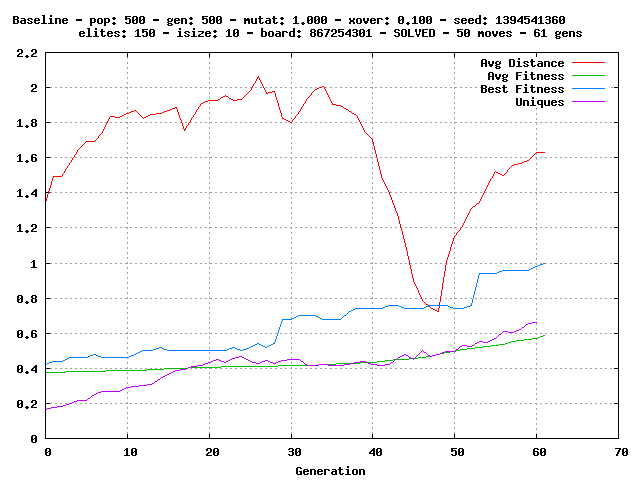
\includegraphics{img/1.png} 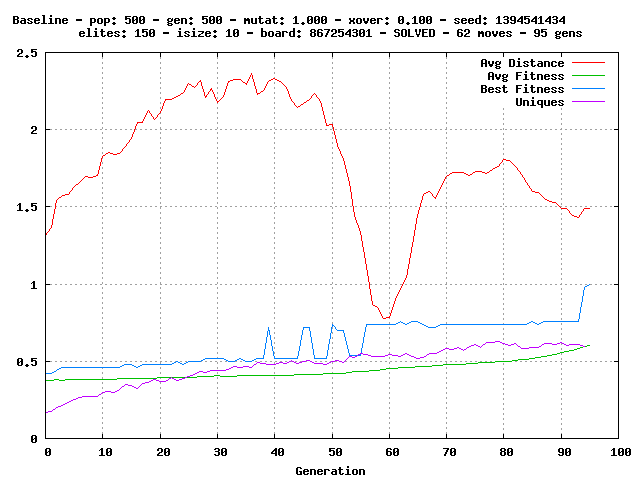
\includegraphics{img/2.png}
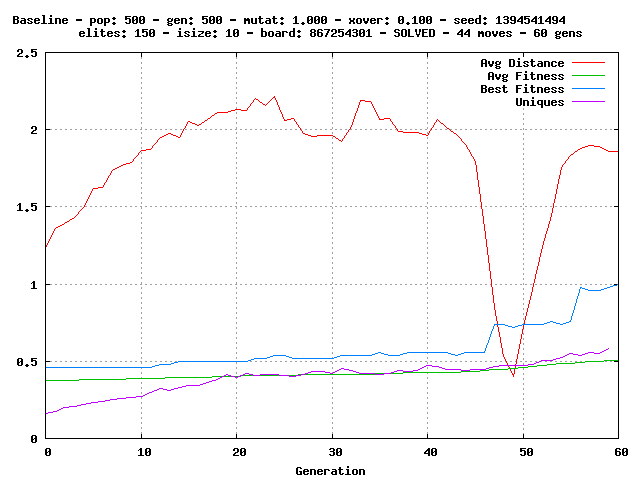
\includegraphics{img/3.png} 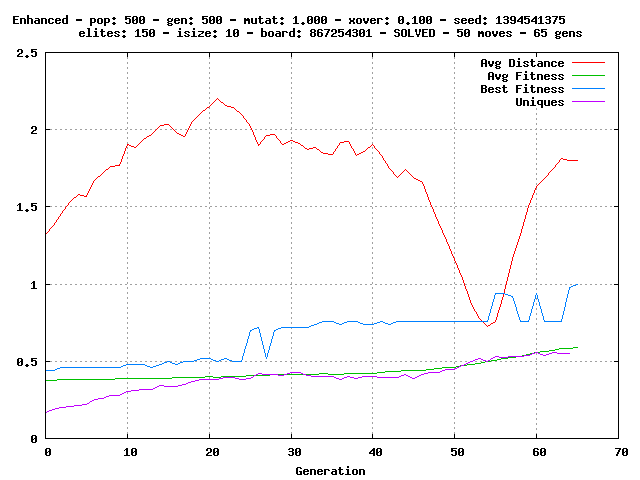
\includegraphics{img/4.png}
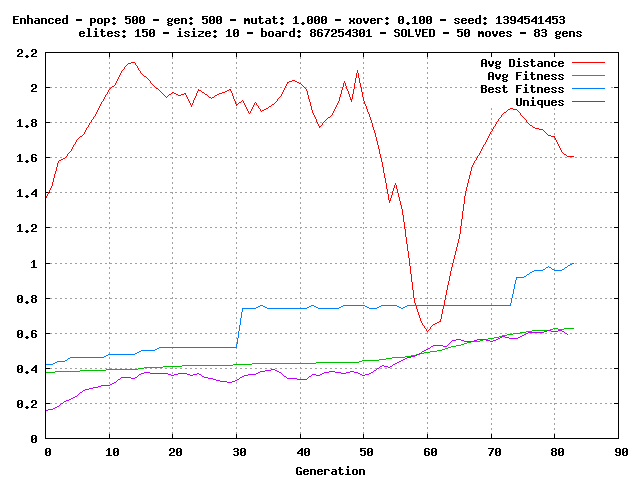
\includegraphics{img/5.png} 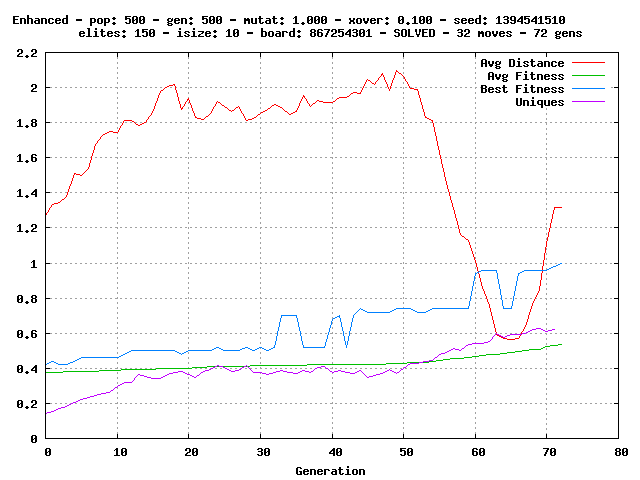
\includegraphics{img/6.png}

\section{Results}\label{results}

Both GAs were able to find solutions for each run that was given to
them. The diversity was increased more rapidly in the ENGA as was
expected. The ENGA outperformed the BLGA in the average size of the
solution by eight moves. The ENGA underperformed the BLGA in the average
number of generations to find solution by 12.33.

\section{Analysis}\label{analysis}

In the BLGA diversity control was never a problem. This may be because
of the design of the GA or the simplicity of the problem. Perhaps if the
GA were designed to find the shortest solution, diversity control may be
more necessary.

The ENGA performed fairly well in comparision to the BLGA. The added
computational complexity of the first method of diversity calculation
being O(N\^{}2) was too much for quick experimentation. The uniqueness
method that was used for diversity control may be a little to simplistic
for robust control of a GA.

\subsection{Description of Source
Files}\label{description-of-source-files}

\begin{itemize}
\itemsep1pt\parskip0pt\parsep0pt
\item
  \texttt{world.cpp}: Controls the entire run of the GA. Seeds the
  initial population and houses all control parameters.
\item
  \texttt{population.cpp}: The data structure for holding the solutions.
  Allows the wholesale calling of growth and mutation on solutions.
\item
  \texttt{solution.cpp}: The chromosome data structure for each
  solution. Methods include mutation and crossover as well as auxiliary
  methods for getting and checking details of a solution.
\item
  \texttt{board.cpp}: The gene data structure for each puzzle state. The
  encoding and decoding of each puzzle into an integer and array are
  located in this file. Logic for movement of tiles and fitness
  calculations are also located here.
\item
  \texttt{main.cpp}: Parses command line arguments and creates the
  world.
\end{itemize}

\end{document}
